%\subsection{Histogramm f\"ur Evaluation Guideline (76)}
%\begin{figure}
\begin{center}
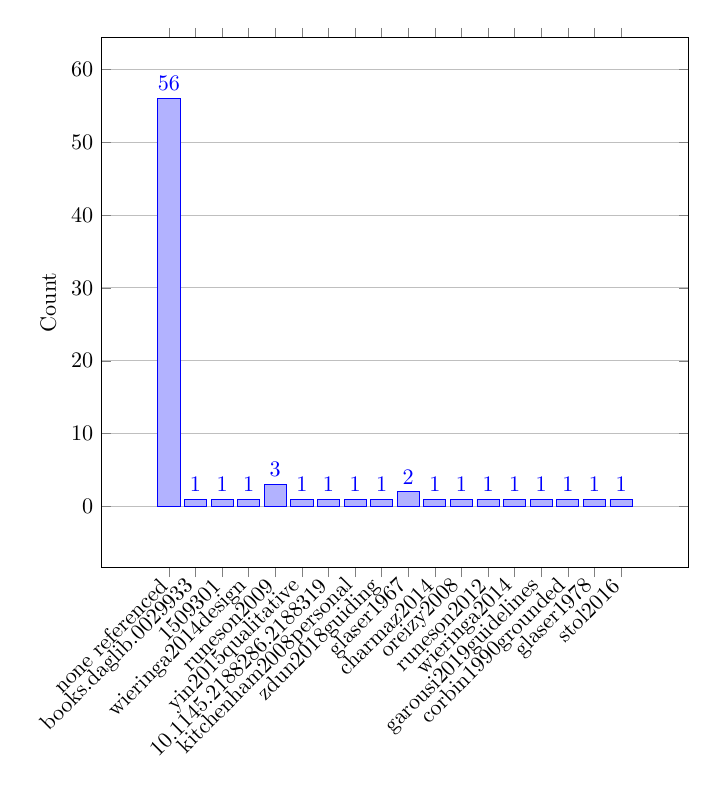
\begin{tikzpicture}[scale=.8]
\begin{axis}[ ybar, ymajorgrids, enlargelimits=0.15, legend style={at={(0.5,-0.15)}, anchor=north,legend columns=-1},
    width=.90\linewidth,height=10cm,
    nodes near coords, %nodes near coords align=below,
    ylabel={Count}, ymin=0,
    x tick label style={rotate=45,anchor=east},
    xtick={1,2,3,4,5,6,7,8,9,10,11,12,13,14,15,16,17,18},
    xticklabels={ none referenced, books.daglib.0029933, 1509301, wieringa2014design, runeson2009, yin2015qualitative, 10.1145.2188286.2188319, kitchenham2008personal, zdun2018guiding, glaser1967, charmaz2014, oreizy2008, runeson2012, wieringa2014, garousi2019guidelines, corbin1990grounded, glaser1978, stol2016
}
    %xlabel={Evaluation Guideline}    
    ]
  \addplot coordinates { (1,56)  (2,1)  (3,1)  (4,1)  (5,3)  (6,1)  (7,1)  (8,1)  (9,1)  (10,2)  (11,1)  (12,1)  (13,1)  (14,1)  (15,1)  (16,1)  (17,1)  (18,1)   };
\end{axis}
\end{tikzpicture}
\end{center}
%\caption{Histogramm f\"ur Evaluation Guideline (76)}
%\label{fig:histo_evaluationguideline}
%\end{figure}

